% !TEX root =  ../main_manuscript.tex

\section{Methods}
\label{sec:methods}
\subsection{Study Population}
To develop our methodology we use data of the patients of the PRIAS study (\url{www.prias-project.org}). The dataset consists of 5270 patients, of which 866 observe cancer progression. For each patient, PSA measurements (ng/mL) are scheduled every 3 months for the first 2 years and every 6 months thereafter. The DRE measurements are scheduled every 6 months. We use the DRE measurements after converting them on a binary scale, namely $\mbox{DRE} > \mbox{T1c}$ and $\mbox{DRE} \leq \mbox{T1c}$ \cite{schroder1992tnm}. On average 5 DRE and 9 PSA measurements have been recorded per patient. In order to identify cancer progression, biopsies are scheduled as per the PRIAS protocol (see \hyperref[sec:introduction]{Introduction}).

\subsection{A Bivariate Joint Model for the Longitudinal PSA, and DRE Measurements, and Time to Cancer Progression}
Let $T_i^*$ denote the true cancer progression time for the $i$-th patient in PRIAS. Since biopsies are conducted periodically, $T_i^*$ cannot be observed directly and it is only known to fall in an interval ${l_i < T_i^* \leq r_i}$, where $r_i$ and $l_i$ are the time of the latest and second latest biopsies, respectively, if the progression is observed at the latest biopsy. When the progression is not observed, then $l_i$ is the time of the latest biopsy and $r_i = \infty$. Further, let $\boldsymbol{y}_{di}$, and $\boldsymbol{y}_{pi}$ denote the $n_{di} \times 1$, and $n_{pi} \times 1$ vectors of the DRE, and PSA longitudinal measurements, respectively. For a sample of $n$ patients the observed data is denoted by ${\mathcal{D}_n = \{l_i, r_i, \boldsymbol{y}_{di}, \boldsymbol{y}_{pi}; i = 1, \ldots, n\}}$.

The patient-specific PSA and DRE measurements over time are modeled using a generalized linear mixed effects model. For the $i$-th patient, the mixed effects sub-model for DRE is given by:
\begin{equation}
\label{eq:long_model_dre}
\begin{split}
    \mbox{logit} \big[\mbox{Pr}\{y_{di}(t) > \mbox{T1c}\}\big] &= \beta_{0d} + b_{0di} + (\beta_{1d} + b_{1di}) t\\
    &+ \beta_{2d} (\mbox{Age}_i-70) + \beta_{3d} (\mbox{Age}_i-70)^2
    \end{split}
\end{equation}
where, $t$ denotes a specific time point in the AS follow-up, $\mbox{Age}_i$ is the age of the $i$-th patient at the time of inclusion in AS. The fixed effect parameters are denoted by $\{\beta_{0d}, \ldots, \beta_{3d}\}$, and $b_{0di}, b_{1di}$ are the patient specific random effects. With this definition, we assume that the log odds of obtaining a DRE score larger than T1c remain linear over time. An example model fit for DRE is shown in panel A of Figure~\ref{fig:jmExplanationPlot_1757}. For the $i$-th patient, the mixed effects sub-model for PSA is given by:
\begin{equation}
\label{eq:long_model_psa}
\begin{split}
    \log_2 \big\{y_{pi}(t) + 1\big\} &= m_{pi}(t) + \varepsilon_{pi}(t),\\
    m_{pi}(t) &= \beta_{0p} + b_{0pi} + \sum_{k=1}^4 (\beta_{kp} + b_{kpi})  B_k(t,\mathcal{K})\\ 
    &+ \beta_{5p} (\mbox{Age}_i-70) + \beta_{6p} (\mbox{Age}_i-70)^2,
    \end{split}
\end{equation}
where, $m_{pi}(t)$ denotes the underlying measurement error free value of $\log_2 (\mbox{PSA} + 1)$ transformed \citep{pearson1994mixed,lin2000latent} measurements at time $t$. To accommodate for a non-linear evolution of this value over the follow-up period in AS, we utilize B-splines \citep{de1978practical}. In Equation (\ref{eq:long_model_psa}), $B_k(t, \mathcal{K})$ denotes the $k$-th basis function of a B-spline with three internal knots at $\mathcal{K} = \{0.1, 0.7, 4\}$ years, and boundary knots at 0 and 5.42 years (0.95 quantile of the observed follow-up times). The fixed effect parameters are denoted by $\{\beta_{0p},\ldots,\beta_{6p}\}$ and the patient specific random effects are denoted by $\{b_{0pi}, \ldots, b_{4pi}\}$. The error $\varepsilon_{pi}(t)$ is assumed to be t-distributed with three degrees of freedom (see Appendix~B.1) and scale $\sigma$, and is independent of the random effects. An example model fit for PSA is shown in panel B of Figure~\ref{fig:jmExplanationPlot_1757}. To account for the association between the DRE and PSA measurements, we link their corresponding random effects. More specifically, the complete vector of random effects ${\boldsymbol{b}_i = (b_{0di}, b_{0di}, b_{0pi}, \ldots, b_{4pi})^T}$ is assumed to follow a multivariate normal distribution with mean zero and ${7\times 7}$ variance-covariance matrix $\boldsymbol{D}$.
\begin{figure}[!htb]
\captionsetup{justification=justified}
\centerline{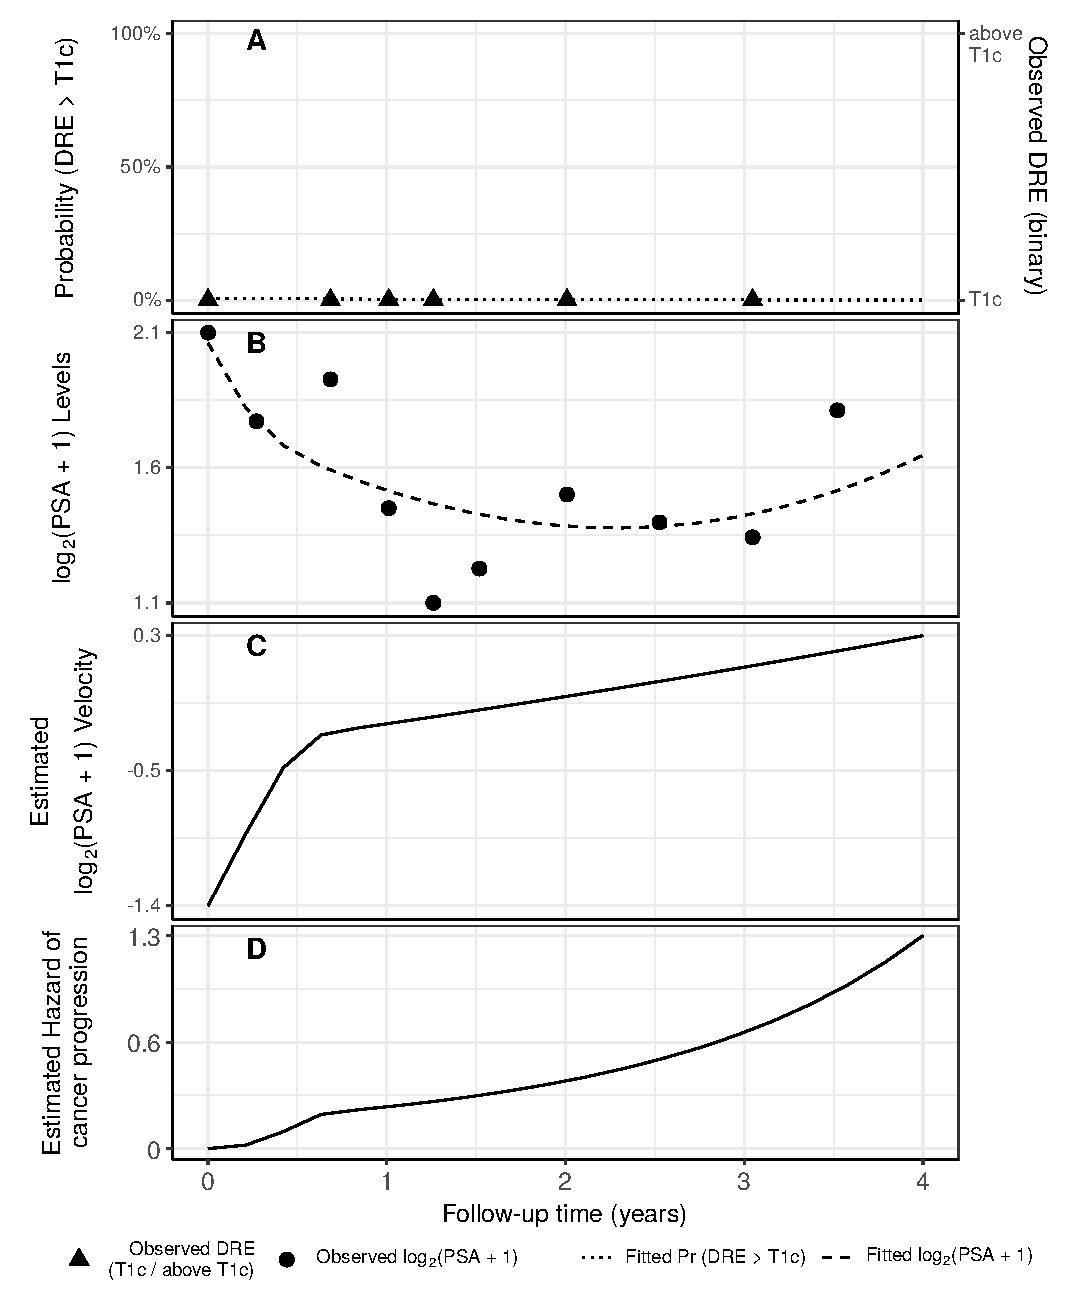
\includegraphics[width=\columnwidth]{images/jmExplanationPlot_1757.eps}}
\caption{Illustration of the joint model fitted to the PRIAS dataset. \textbf{Panel~A:} shows the observed DRE scores and the fitted probability of obtaining a DRE score greater than T1c (Equation~\ref{eq:long_model_dre}). \textbf{Panel~B:} shows the observed and fitted $\log_2(\mbox{PSA} + 1)$ levels (Equation~\ref{eq:long_model_psa}). \textbf{Panel~C:} shows the estimated $\log_2(\mbox{PSA} + 1)$ velocity (velocity cannot be observed directly) over time. The hazard function (Equation~\ref{eq:rel_risk_model}) shown in \textbf{Panel~D}, depends on the fitted log odds of having a $\mbox{DRE} > \mbox{T1c}$, and the fitted $\log_2(\mbox{PSA} + 1)$ value and velocity.}
\label{fig:jmExplanationPlot_1757}
\end{figure}

To model the impact of DRE and PSA measurements on the risk of cancer progression, we use a relative risk sub-model. More specifically, the hazard of cancer progression $h_i(t)$ at a time $t$ is given by:
\begin{equation}
\label{eq:rel_risk_model}
\begin{split}
    h_i(t) &= h_0(t) \exp\Big(\gamma_1 (\mbox{Age}_i-70) + \gamma_2 (\mbox{Age}_i-70)^2\\
    &+\alpha_{1d} \times \mbox{logit} \big[\mbox{Pr}\{y_{di}(t) > \mbox{T1c}\}\big]+ \alpha_{1p} \times m_{pi}(t) + \alpha_{2p} \times \frac{\partial m_{pi}(t)}{\partial {t}}\Big),
    \end{split}
\end{equation}
where, $\gamma_1, \gamma_2$ are the coefficients for the effect of age. The parameter $\alpha_{1d}$ models the impact of log odds of obtaining $\mbox{DRE} > \mbox{T1c}$ on the hazard of cancer progression. The impact of PSA on the hazard of cancer progression is modeled in two ways, namely at any time $t$ the effect of the instantaneous underlying value (dashed line in panel B of Figure~\ref{fig:jmExplanationPlot_1757}) of PSA $m_{pi}(t)$ is given by $\alpha_{1p}$, and the effect of the instantaneous underlying PSA velocity $\partial m_{pi}(t)/\partial {t}$ (panel C in Figure~\ref{fig:jmExplanationPlot_1757}) is given by $\alpha_{2p}$. Lastly, $h_0(t)$ is the baseline hazard at time $t$, and is modeled flexibly using P-splines \citep{eilers1996flexible}. An example fitted hazard is shown in Panel D of Figure~\ref{fig:jmExplanationPlot_1757}. The detailed specification of the baseline hazard $h_0(t)$, and parameter estimation using the Bayesian approach are presented in Appendix A of the supplementary material.

\subsection{Personalized Decisions for Biopsy During Follow-up Visit}
\label{subsec:pers_decision_making}
Let us assume that a decision of conducting a biopsy is to be made for a new patient $j$, who is not present in the PRIAS dataset. Let $t$ be the time of his latest biopsy, and $s$ denotes the current follow-up visit time. Let $\mathcal{Y}_{dj}(s)$ and $\mathcal{Y}_{pj}(s)$ denote the vector of all DRE and PSA measurements taken up to the current visit $s$, respectively. From the observed measurements we want to extract the underlying measurement error free trend of $\log_2 (\mbox{PSA} + 1)$ values and velocity, and the log odds of obtaining $\mbox{DRE} > \mbox{T1c}$. We intend to combine them to inform us when the cancer progression is to be expected (see Figure~\ref{fig:dynRiskPlot_2340}), and to further guide the decision making on whether to conduct a biopsy at the current follow-up visit. The combined information is given by the posterior predictive distribution $g(T^*_j)$ of the time of cancer progression $T^*_j$. It is given by:
\begin{equation*}
\label{eq:post_pred_dist}
\begin{aligned}
g(T^*_j) &= p\big\{T^*_j \mid T^*_j > t, \mathcal{Y}_{dj}(s), \mathcal{Y}_{pj}(s), \mathcal{D}_n\big\}\\
&= \int \int p\big(T^*_j \mid T^*_j > t, \boldsymbol{b}_j, \boldsymbol{\theta}\big)\\
&\times p\big\{\boldsymbol{b}_j \mid T^*_j>t, \mathcal{Y}_{dj}(s), \mathcal{Y}_{pj}(s), \boldsymbol{\theta}\big\}p\big(\boldsymbol{\theta} \mid \mathcal{D}_n\big) \mathrm{d} \boldsymbol{b}_j \mathrm{d} \boldsymbol{\theta}.
\end{aligned}
\end{equation*}
The distribution $g(T^*_j)$ updates as extra information is recorded at follow-up visits. It is also unique for each patient as it depends on the historical data of the patient via the posterior distribution of the random effects $\boldsymbol{b}_j$.

A key ingredient in the decision of conducting a biopsy at the current follow-up visit time $s$, is the risk that the cancer has already progressed since the time of the last biopsy $t$ (see Figure~\ref{fig:dynRiskPlot_2340} for illustration). This risk can be derived from the posterior predictive distribution $g(T^*_j)$ \cite{rizopoulos2011dynamic}, and is given by:
\begin{equation*}
\label{eq:dynamic_risk_prob}
R_j(s \mid t) = \mbox{Pr}\big\{T^*_j \leq s \mid T^*_j > t, \mathcal{Y}_{dj}(s), \mathcal{Y}_{pj}(s), \mathcal{D}_n\big\}, \quad s \geq t.
\end{equation*}
\begin{figure}[!htb]
\captionsetup{justification=justified}
\centerline{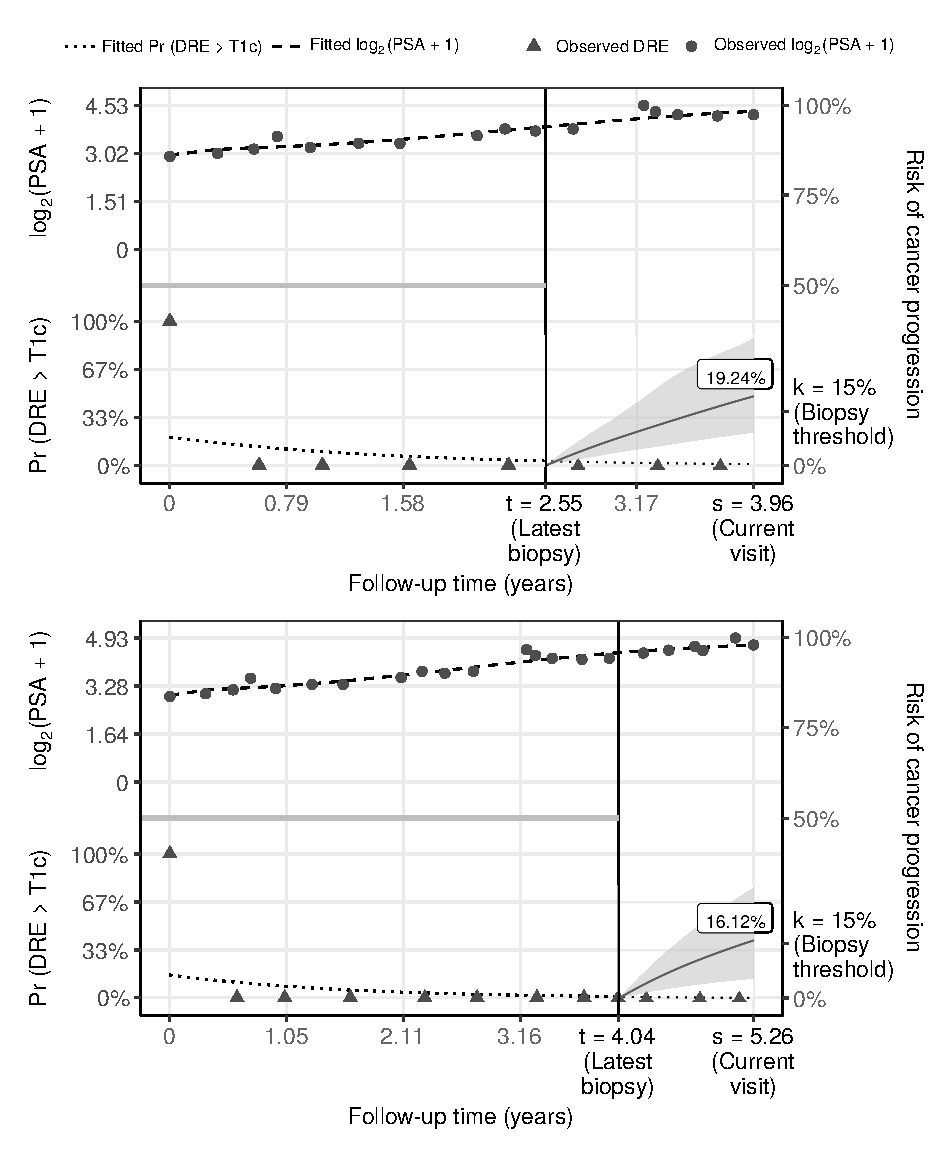
\includegraphics[width=\columnwidth]{images/dynRiskPlot_2340.eps}}
\caption{Illustration of personalized decision making for patient $j$ at two different follow-up visits. Biopsy is recommended if the risk of cancer progression estimated from the joint model fitted to the PSA and DRE measurements of the patient, is higher than the example risk threshold for biopsy ($\kappa=$ 15\%). \textbf{Panel~A:} biopsy is not recommended for the patient $j$ at the follow-up visit time $s=4$ years, because his estimated risk of cancer progression (10.2\%) is less than the biopsy risk threshold. \textbf{Panel~B:} biopsy is recommended for the patient $j$ at the follow-up visit time $s=5.3$ years, because his estimated risk of cancer progression (17.8\%) is more than the biopsy risk threshold.}
\label{fig:dynRiskPlot_2340}
\end{figure}
A simple and straightforward approach to decide upon conducting a biopsy at a follow-up visit would be to do so when the risk of cancer progression at that visit is higher than a certain threshold $0 \leq \kappa \leq 1$. For example, as shown in panel B of Figure~\ref{fig:dynRiskPlot_2340}, biopsy at a follow-up visit may be scheduled if the risk is higher than 15\% (example risk threshold). Since there are infinite possible risk thresholds between 0\% and 100\% risk, the choice of a single threshold at a follow-up visit can become dilemmatic for patients/doctors.

In such situations, we propose an alternative approach of automatic selection of thresholds. Using information from the observed cancer progression times in the PRIAS dataset, at a follow-up visit a threshold is chosen on the basis of its ability to discriminate between patients who obtain cancer progression versus others. More specifically, given the time $t$ of the latest biopsy we propose to choose a threshold $\kappa$ for which a binary classification accuracy measure \citep{lopez2014optimalcutpoints}, discriminating between patients observing cancer progression (positive result) versus others (negative result), is maximized. In joint models, a patient $j$ is predicted to have progression in the time period $(t, s]$ between the current visit and the last biopsy, if ${R_j(s \mid t) > \kappa}$ \cite{rizopoulosJMbayes, landmarking2017}. Otherwise the patient is predicted to not have progression. Since we are interested in detecting cancer progressions, we can choose a $\kappa$ for which the true positive rate (also known as sensitivity, or probability of detection) is maximized. However, this may lead to a high false positive rate as well (unnecessary biopsy suggestions). This issue can be mitigated by maximizing for the positive predictive value (also known as precision) simultaneously. To this end, we utilize the $\mbox{F}_1$ score, which is a composite of time dependent true positive rate (TPR) and positive predictive value (PPV), and is defined as:
\begin{equation}
\label{eq:F1_TPR_PPV}
\begin{split}
\mbox{F}_1(t,  s, \kappa) &= 2\frac{\mbox{TPR}(t,  s, \kappa)\ \mbox{PPV}(t,  s, \kappa)}{\mbox{TPR}(t,  s, \kappa) + \mbox{PPV}(t,  s, \kappa)},\\
\mbox{TPR}(t,  s, \kappa) &= \mbox{Pr}\big\{R_j(s \mid t) > \kappa \mid t < T^*_j \leq s\big\},\\
\mbox{PPV}(t,  s, \kappa) &= \mbox{Pr}\big\{t < T^*_j \leq s \mid R_j(s \mid t) > \kappa \big\}.
\end{split}
\end{equation}
The $\mbox{F}_1$ score ranges between 0 and 1, where a value of 1 signifies perfect TPR and PPV. Since a high $\mbox{F}_1$ score is desired, the value of biopsy threshold $\kappa$ is $\argmax_{\kappa} \mbox{F}_1(t, s, \kappa)$. The time dependent TPR and PPV are estimated from the joint model fitted to the PRIAS dataset \cite{landmarking2017}.

\subsection{Simulation Study}
Although the personalized decision making approach is motivated by the PRIAS study, it is not possible to evaluate it on the PRIAS dataset. This is due to the fact that the PRIAS patients have already had their biopsies as per the PRIAS protocol. In addition, the true time of cancer progression is interval or right censored for all patients, making it impossible to correctly estimate the delay in detection of cancer progression due to a particular schedule. To this end, we conduct an extensive simulation study to compare personalized, PRIAS and annual schedules. For a realistic comparison, we simulate data from the joint model fitted to the PRIAS dataset. The simulated population has the same follow-up period of 10 years as the PRIAS study. In addition the recovered relations between PSA and DRE measurements, and the risk of cancer progression, are retained in the simulated population.

From this population, we first sample 500 datasets with 1000 patients each. We generate a true cancer progression time for each of the patients, and then sample a set of PSA and DRE measurements at the same time points as given in PRIAS protocol. We then split each dataset into a training (750 patients) and a test (250 patients) part, and generate a random and non‐informative censoring time for the training patients. We next fit a joint model of the specification given in Equation (\ref{eq:long_model_dre}), (\ref{eq:long_model_psa}) and (\ref{eq:rel_risk_model}) to each of the 500 training datasets and obtain MCMC samples from the 500 sets of the posterior distribution of the parameters. Using these fitted joint models, we obtain the posterior predictive distribution of time of cancer progression for each of the 500$\times$250 test patients at each of their visits. While maintaining a gap of 1 year between consecutive biopsies, for each patient at each follow-up visit we make the decision of (not) conducting a biopsy. 

In this simulation study, during follow-up visits we make the decision of biopsies as per the following approaches (abbreviated names in parenthesis): biopsy every year (Annual), biopsy as per the PRIAS protocol (PRIAS), personalized biopsy using: a risk threshold of 5\% (Risk: 5\%), risk threshold of 15\% (Risk: 15\%), and risk threshold chosen automatically by maximizing $\mbox{F}_1$ score (Risk: Automatic). In addition, in each of the aforementioned approaches, one biopsy each is conducted at the time of inclusion in  AS (year 0) and at the end (year 10) of the follow-up period. This results into an entire personalized schedule for each patient. We compare the resulting biopsy schedules on two measures, namely the number of biopsies they schedule and the delay in detection of cancer progression incurred due the schedule. We define the delay as the difference between the time of the biopsy on which cancer progression is detected and the true time of cancer progression. Ideal numbers for these two measures are 1 biopsy and 0 years of delay.